\section{Introduction to Physics}

\begin{multicols}{2}


\section*{Concept of Physics}


%\subsection{•}

\begin{center}
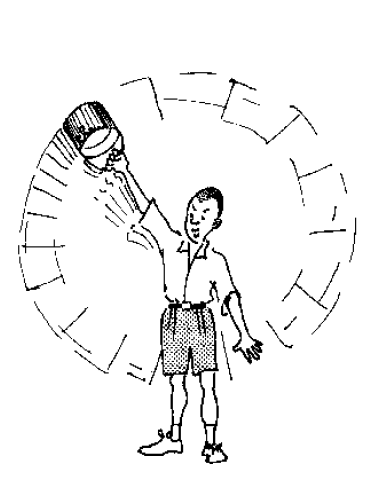
\includegraphics[width=0.45\textwidth]{./img/source/bucket-swing-2.png}
\end{center}

%\begin{description*}
%%\item[Subtopic:]{}
%\item[Materials:]{}
%\item[Setup:]{}
%\item[Procedure:]{}
%\item[Hazards:]{}
%\item[Questions:]{}
%\item[Observations:]{}
%\item[Theory:]{}
%\item[Applications:]{}
%\item[Notes:]{}
%\end{description*}

A bucket of water is sufficient to start investigating the effect of centripetal forces. Fill the
bucket with various quantities of water and you will learn even more by doing. Increase the
number of revolutions of the bucket.\\

Physics must not be a boring, tough subject, just good for exams and to be understood by a
few ``experts'' only. Physics should not happen in books only. It is everywhere where things
are. The teaching of science without experiments is just like a ngoma without dancers.\\

Pupils learn more and better by doing. Stimulate them to investigate their environment
through easy to carry out experiments. Ask the pupils to make a list of physical phenomena
which can be observed in their environment. Let the pupils enjoy physics. The activities in this book
show how this can be achieved.

\vfill
\columnbreak


%==================================================================================================%

\section*{Applications of Physics}


\subsection{Measurement and Data}

\begin{center}
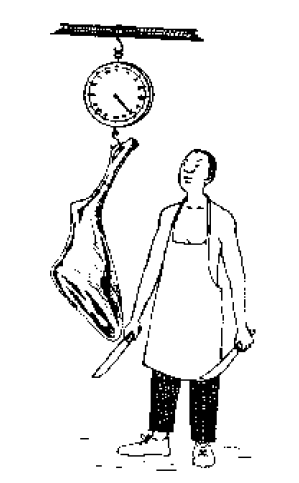
\includegraphics[width=0.4\textwidth]{./img/source/butcher.png}
\end{center}

Imagine you would buy different kinds and different quantities of meat. The butcher will have
to weigh and then calculate the price for each kind of meat and produce the total bill. Thus,
measuring and the collection of data happen everyday in our life.\\

The tailor takes the measurements of his customer and of the material needed for a suit. The
milkman measures the volume of the milk sold. The technician measures with a caliper the
diameter of a screw and even at school the time of each period is measured. Especially in
engineering precise measurements are indispensable.

\vfill
\columnbreak

\subsection{Mechanics}

\begin{center}
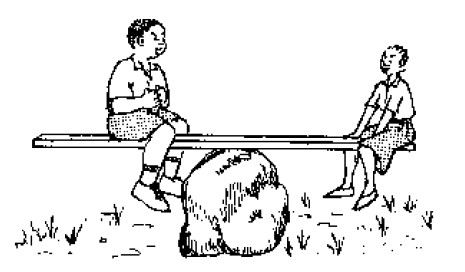
\includegraphics[width=0.4\textwidth]{./img/source/mechanics.png}
\end{center}

Have you observed children balancing a plank like a seesaw? They know how a big and a
small child can balance although they are of different weight.\\

Usually they do not know what a fulcrum, a load distance and a moment of force is. However,
such basic mechanics dominate an essential part of our daily life. We encounter motion,
friction, inertia, work and power almost every day. We also learn in a practical way about
density, pressure of fluids or gases. Work, energy, power and other physical phenomena look
very abstract in books but happen every day. Also the movement of earth, moon and the
planets which determines the lengths of our days, months and years, has to do with basic
mechanics such as motion, mass attraction and centripetal forces.

\subsection{Matter}

\begin{center}
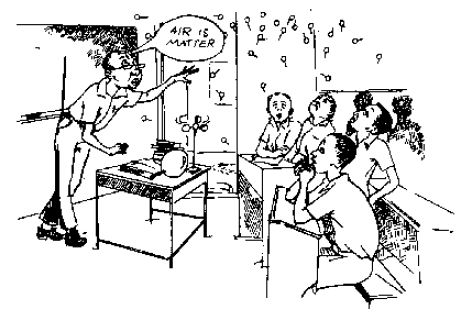
\includegraphics[width=0.4\textwidth]{./img/source/matter.png}
\end{center}

A chair can be touched. Water in a bucket also. But air? Can you imagine that while you are
reading these lines your nose is punched more than 100 billion times by air molecules?\\

The environment around us, whether in solid, liquid or gaseous state is made up of billions of
tiny particles which are either molecules or atoms. These particles which constitute air are so
tiny, that we cannot see them even by a powerful microscope. However, the students can be
given an idea of the particle structure of matter by indirect evidence.

\subsection{Thermal Physics}

\begin{center}
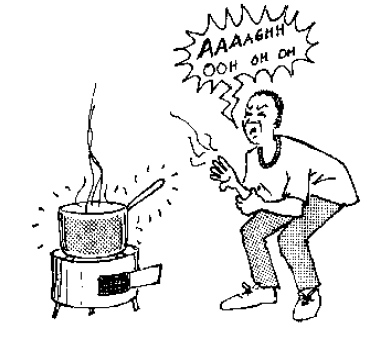
\includegraphics[width=0.4\textwidth]{./img/source/thermal-physics.png}
\end{center}

Would you ever touch the handle of a hot pan? Would you put margarine just aside
of the pot? Would you hold your hand right above the hot water? No; this is
because we know a lot about thermal physics by daily experience. But we do not always
relate this knowledge with what we learn at school about heat conduction, heat radiation or
heat convection as is the case in the examples mentioned above.\\

Thermal physics has also to do with thermal energy and the measurement of temperatures,
with calorimetry, change of states, expansion, etc. Ask the students to talk about everyday
thermal phenomena and to write about these. Why should we teach this topic by talk and
chalk only, if there are illustrative experiments which do not require a lot of equipment and
which are not time consuming in their preparation and performance?

\subsection{Wave Motion}

\begin{center}
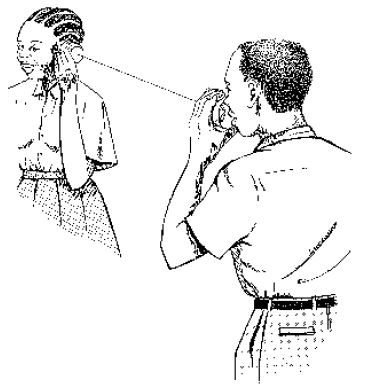
\includegraphics[width=0.4\textwidth]{./img/source/wave-motion.jpg}
\end{center}

Communication through spoken words has to do with the transport of waves. Telephone and
radio are well known. But do we think about waves when we hear a music band, when a crow
is croaking or when children are playing with a string telephone? All this is everyday knowledge about the transport of sound waves.\\

But teaching about waves does not mean only sound waves. Water waves we notice in a puddle as well as in a cup of tea. Electromagnetic waves are responsible for hearing our radios and watching our televisions.
Produce waves in physics not only by talking. Meaningful and simple experiments are
possible on many themes of this topic. No time? Hand experiments are always brief,
illustrative and can be carried out with everyday things.

\subsection{Light and Optics}

\begin{center}
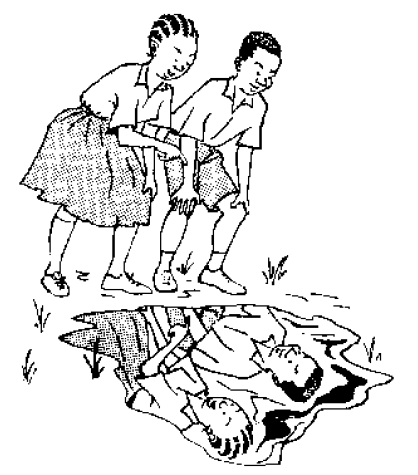
\includegraphics[width=0.4\textwidth]{./img/source/light-optics.png}
\end{center}

When we hear about optics, the optician, eye glasses and lenses come into our mind. But that
is not all what optics is about. Optics is also about the reflection of an image in a mirror or in a
water puddle. The water surface is like a mirror. The image to be seen is inverted and it
seems to be as far behind the water surface as the object is in front of it.\\

Perhaps there are no curved mirrors at your school to teach about concave and convex mirrors. No problem. Take a polished spherical spoon and you will be able to perform an interesting lesson. Certainly not all themes can be taught by simple qualitative hand experiments only. But you may be astonished to see how many there are for eye catching demonstrations.

\subsection{Electricity and Magnetism}

\begin{center}
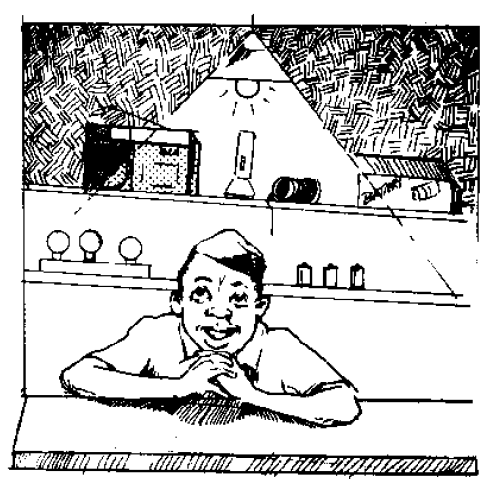
\includegraphics[width=0.4\textwidth]{./img/source/elec-mag.png}
\end{center}

Effects of electricity can be observed nowadays nearly everywhere. A light bulb lights the
room; a radio enchants our ears; a torch helps to find our way in the darkness; and last but
not least we do owe a cool soft drink to a refrigerator. The understanding on how electric
apparatus work is essential nowadays.\\

But electricity does not only mean a current flows in a circuit. It means also static electricity or lightning during a thunderstorm. The topic of electricity is closely related to magnetism.
Without magnets electric motors would not work. Loudspeakers work with magnets and even
a simple bicycle dynamo has one. In harbours you can see how ``attractive'' magnets can be
to lift heavy loads. Do you think that the teaching of electricity by doing is difficult, needs a lot
of equipment and is even dangerous? See that this is not the case by trying some of the activities provided in this manual.

%==================================================================================================%


\end{multicols}

\pagebreak